\section{Tipos de sensores}
\vspace{10mm}
\textbf{Por posición:}
\vspace{5mm}

\textbf{Encoder Incremental :} 

Este tipo de sensor óptico digital convierte el movimiento en una secuencia de pulsos digitales. Tiene una escala transparente con una retícula opaca; de un lado, tiene una escala equipada con una fuente de luz y un lente condensador. Del otro lado, hay celdas sensibles a la luz. La manera en la que funciona es que la resistencia de las celdas disminuye cada vez que reciben un rayo de luz, de este modo se genera un pulso cada vez que un rayo de luz es atravesado.


\begin{figure}[h]
	\centering
	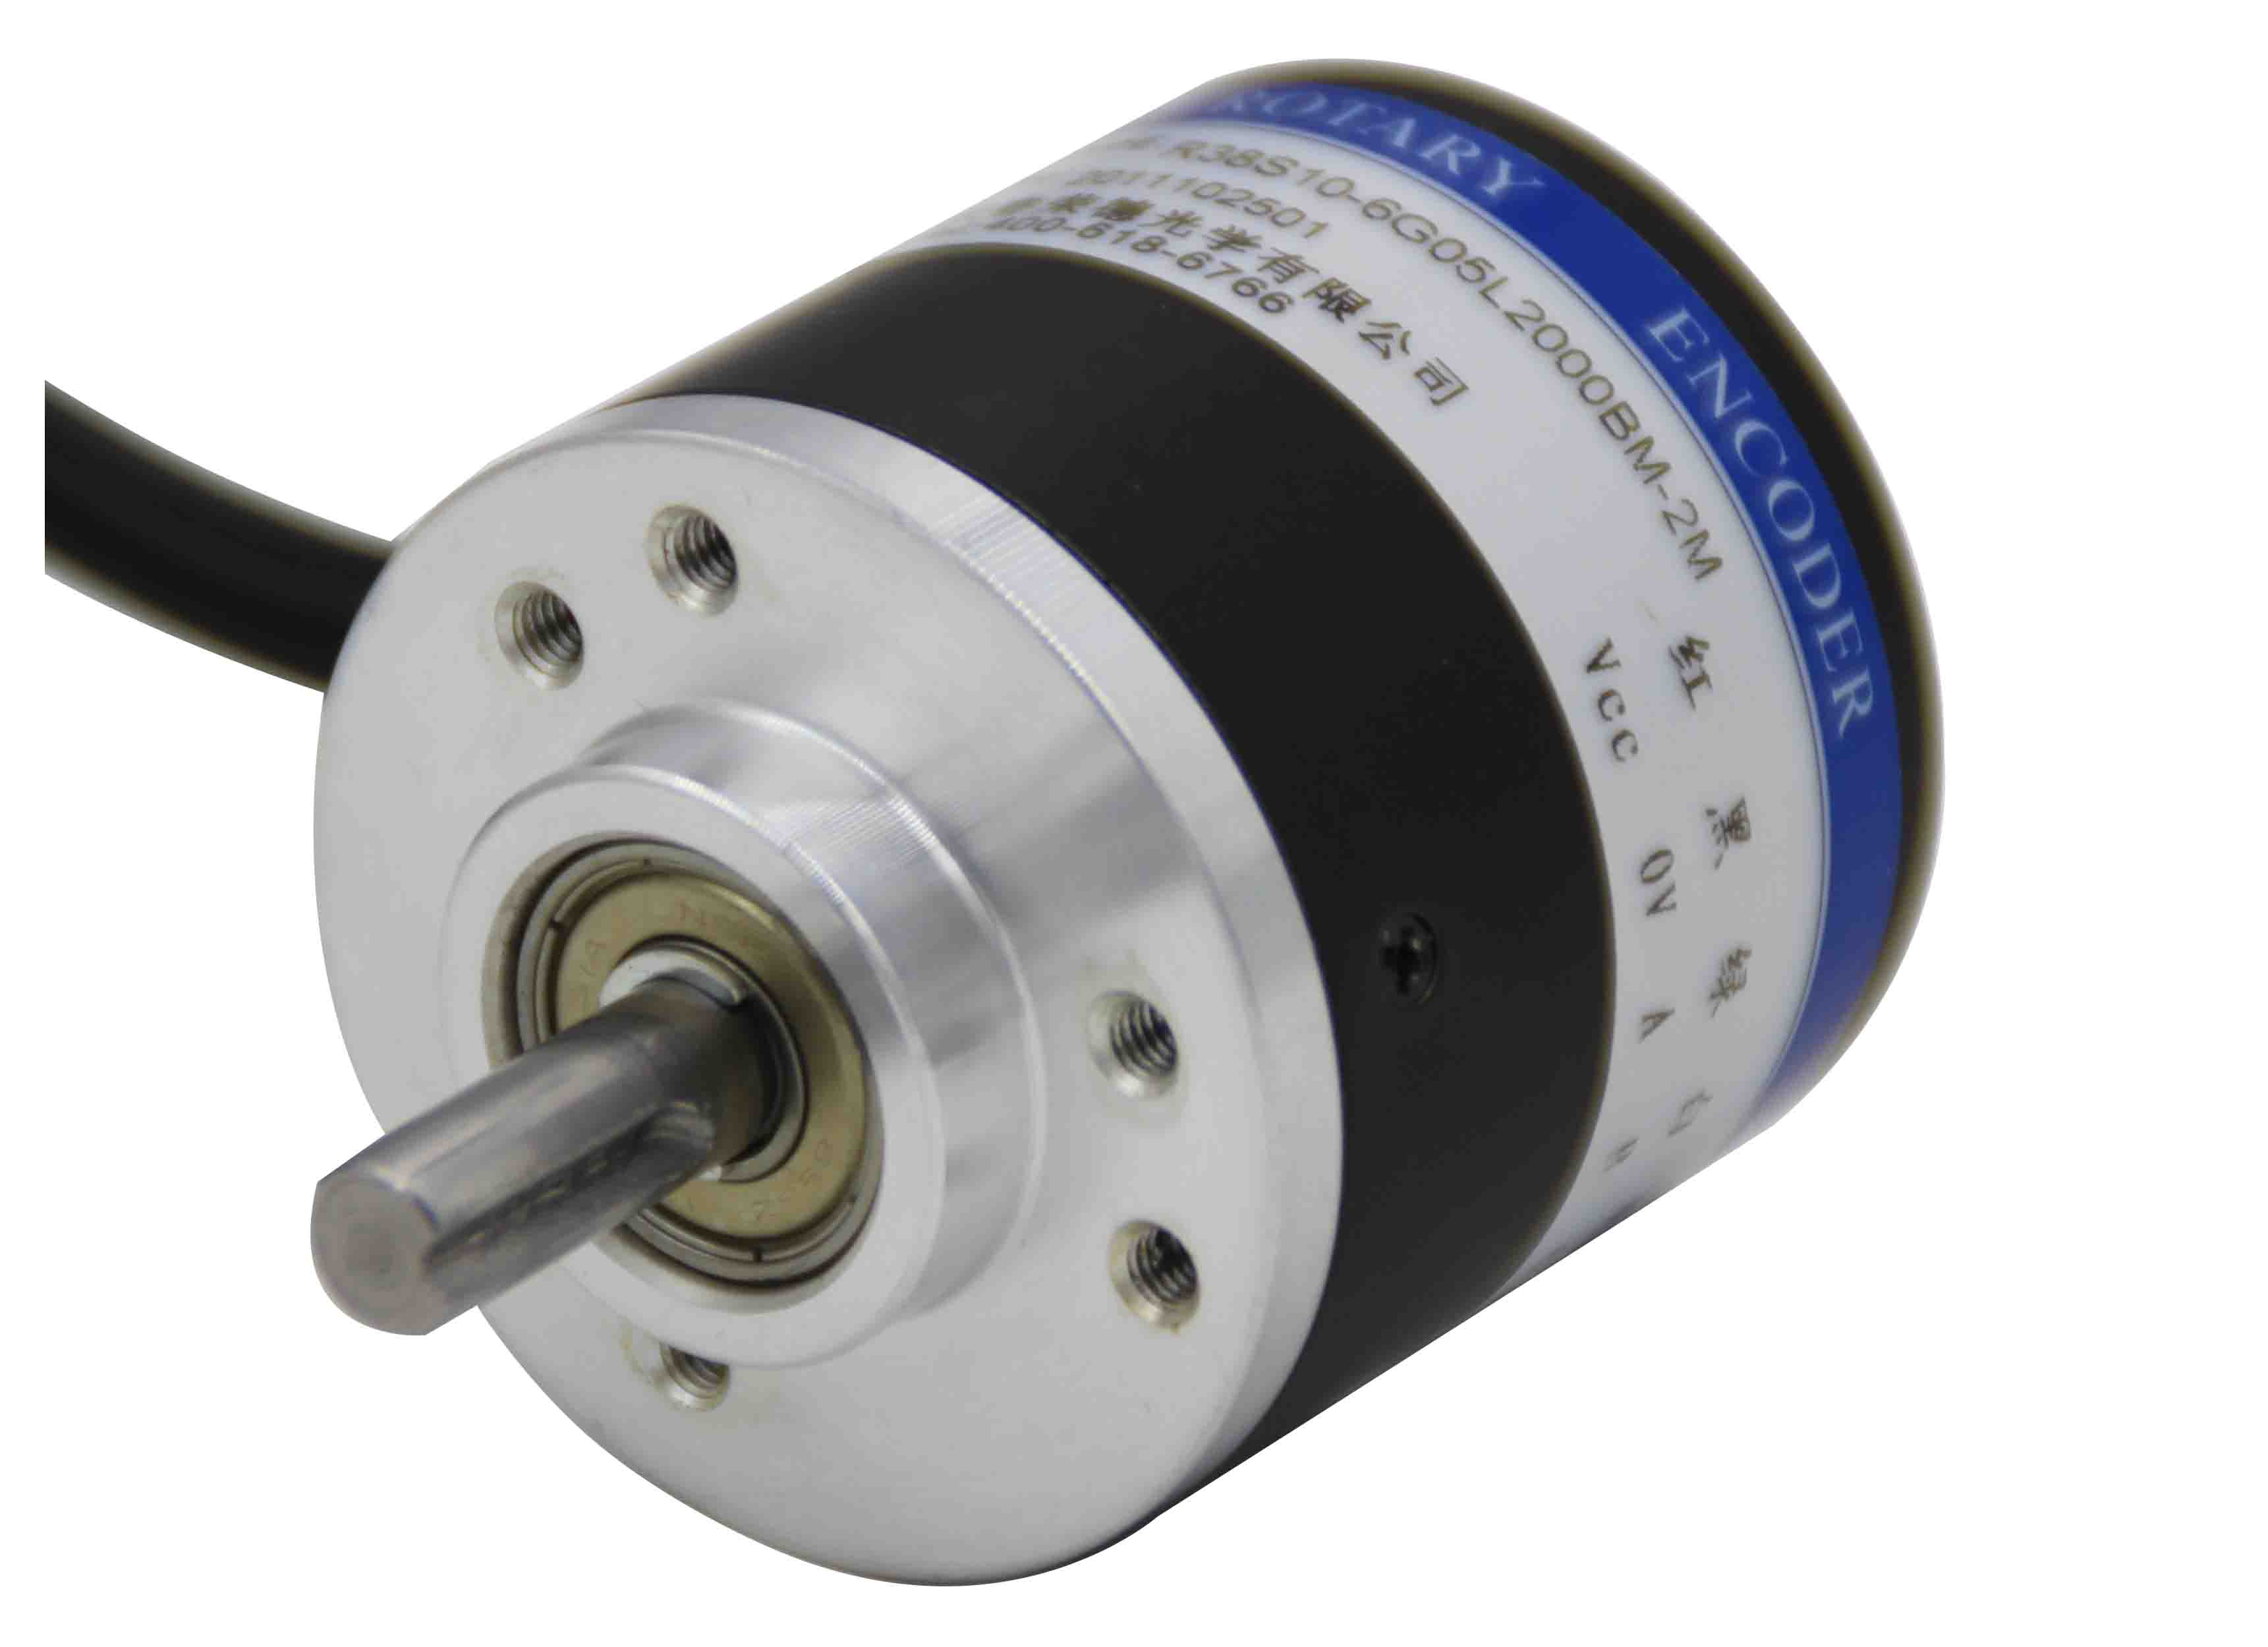
\includegraphics[width=0.4\linewidth]{portada/20150317193931229}
	\caption{Encoder incremental}
	\label{fig:20150317193931229}
\end{figure}

\begin{figure}[h]
	\centering
	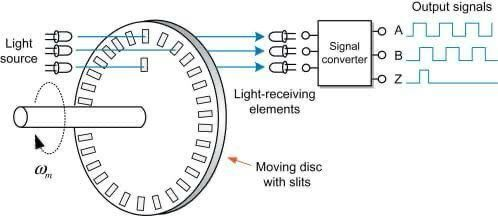
\includegraphics[width=0.4\linewidth]{img/Sencoderincremental}
	\caption{Codificador rotatorio incremental - OMCH}
	\label{fig:Sencoderincremental}
\end{figure}
\vspace{10mm}
\textbf{Encoder Absoluto :} 


\newpage  % Salto de página forzado


